%%%%%%%%%%%%%%%%%%%%%%%%%%%%%%%%%%%%%%%%%
% This template has been downloaded from:
% http://www.LaTeXTemplates.com
%
% Original author:
% WikiBooks (http://en.wikibooks.org/wiki/LaTeX/Title_Creation)
%%%%%%%%%%%%%%%%%%%%%%%%%%%%%%%%%%%%%%%%%
%\title{Title page with logo}
%--------------------------------------------------------------
%	PACKAGES AND OTHER DOCUMENT CONFIGURATIONS
%-------------------------------------------------------------

\documentclass[12pt]{article}
\usepackage[english]{babel}
\usepackage[utf8x]{inputenc}
\usepackage{amsmath}
\usepackage{graphicx}
\usepackage[colorinlistoftodos]{todonotes}

\usepackage{fancyhdr} % Required for custom headers
\usepackage{lastpage} % Required to determine the last page for the footer
\usepackage{extramarks} % Required for headers and footers
\usepackage{lipsum} % Used for inserting dummy 'Lorem ipsum' text into the template
\usepackage{bm}
\usepackage{float}
\usepackage{mathtools}
\usepackage{enumerate}
\usepackage{amssymb}
\usepackage{booktabs}

% Margins
\topmargin=-0.45in
\evensidemargin=0in
\oddsidemargin=0in
\textwidth=6.5in
\textheight=9.0in
\headsep=0.25in 

\linespread{1.1} % Line spacing

% Set up the header and footer
\pagestyle{fancy}
\lhead{}
\chead{Spam Email Classification} % Top center header
\rhead{\firstxmark} % Top right header
\lfoot{\lastxmark} % Bottom left footer
\cfoot{} % Bottom center footer
\rfoot{Page\ \thepage\ of\ \pageref{LastPage}} % Bottom right footer
\renewcommand\headrulewidth{0.4pt} % Size of the header rule
\renewcommand\footrulewidth{0.4pt} % Size of the footer rule

\setlength\parindent{0pt} % Removes all indentation from paragraphs



\begin{document}

\begin{titlepage}

\newcommand{\HRule}{\rule{\linewidth}{0.5mm}} % Defines a new command for the horizontal lines, change thickness here

\center % Center everything on the page
 
%--------------------------------------------------------------
%	HEADING SECTIONS
%--------------------------------------------------------------

\textsc{\LARGE University of California Davis }\\[0.3cm] 
\textsc{\Large Department of Statistics}\\[0.5cm] 
 % Minor heading such as course title

%--------------------------------------------------------------
%	TITLE SECTION
%--------------------------------------------------------------

\HRule \\[0.4cm]
{ \huge \bfseries Machine Learning\\  (STA-208)}\\[0.03cm]
\HRule \\[1.5cm]

\hfill \break \hfill \break \hfill \break
\hfill \break \hfill \break \hfill \break 
\hfill \break \hfill \break \hfill \break
\hfill \break

{\large Ying-Chen Chou \\ Chia-Hui Shen \\Jiahui Tan\\ Pei-Ying Ling}\\


\includegraphics[width=4cm]{logo.png}\\[1cm] 
 
%--------------------------------------------------------------

\vfill % Fill the rest of the page with whitespace

\end{titlepage}

\newpage
\tableofcontents
\newpage
%--------------------------------------------------------------
%Project Start
%--------------------------------------------------------------
\section{Introduction} \label{sec:Intro}

% !TEX root = main.tex
Placeholder for introduction section.


\section{Description of Data} \label{sec:Descript}

\subsection{Data Preprocessing}

There are only a few public sources for email data to which almost everyone trying to do similar analysis will turn to. For our project, we downloaded datasets from the following three locations:

\begin{enumerate}
\item Enron-Spam datasets
\item SpamAssassin data
\item TREC email corpus
\end{enumerate}\\

We combine all emails and extracted the information including date, from, to, subject, content, number of cc, and number of bcc. In the process of data preprocessing, we faced some challenges to get the information of year, weekday, and hour at which the email was sent. We tried to use the string methods in python but end up finding regular expression is more powerful to extract the weekday and month. The other challenge of cleaning up the emails come from trying to remove the html and css elements, such that when we tokenize we wouldn't end up with tag elements as the most frequent words. Although we cannot remove all html and css, we did manage to get rid of most of it by the removal of contents between brackets, parathesis, and curly braces as well as words that begin with a period. \\

\begin{figure}[H]
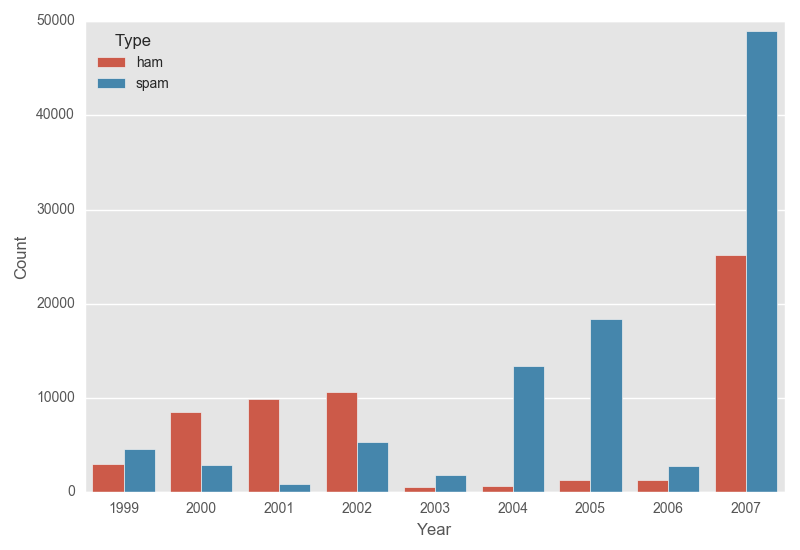
\includegraphics[width=10cm]{Email_count_each_year.png}
\centering
\caption{Amount of Email From 1999 to 2007}
\label{email_every_year}
\end{figure}\\

\begin{table}[h]
\centering
\caption{Proportion of Ham Email and Spam Email From 1999 to 2007}
\label{proportion_ham_spam}
\begin{tabular}{@{}llllll@{}}
\toprule
Year & Ham   & Spam  & Ham \%   & Spam \%  & Total \\ \midrule
1999 & 2978  & 4611  & 0.392410 & 0.607590 & 7589  \\
2000 & 8512  & 2851  & 0.749098 & 0.250902 & 11363 \\
2001 & 9872  & 848   & 0.920896 & 0.079104 & 10720 \\
2002 & 10663 & 5280  & 0.668820 & 0.331180 & 15943 \\
2003 & 545   & 1773  & 0.235116 & 0.764884 & 2318  \\
2004 & 627   & 13420 & 0.044636 & 0.955364 & 14047 \\
2005 & 1309  & 18418 & 0.066356 & 0.933644 & 19727 \\
2006 & 1226  & 2730  & 0.309909 & 0.690091 & 3956  \\
2007 & 25219 & 48999 & 0.339796 & 0.660204 & 74218 \\ \bottomrule
\end{tabular}
\end{table}\\

After finishing the data cleaning up, we delete the emails with year not between 1999 to 2007 to prevent the situation that the date of the emails is after when the data was collected and that the date of email is so early that the email are still not common used. There are 159981 email with 60951 of them are ham and the other 98930 are spam. From Table \ref{proportion_ham_spam} and Figure \ref{email_every_year}, we can see that there is a disproportional number of emails between each year as well as between spam and ham groups. The imbalance dataset may be worrisome for our classifiers. However, there is not much we can do about this situation. Maybe if we can see that there is not too much variation between ham and spam emails across years or there is no time obvious time effect on the emails, then combining the different years wouldn't be a problem. To see whether there are differences in email across the email, we will examine the top words by year. Figure \ref{email_hour_weekday} shown the amount of the email sent each hour and each day. There is a peak for sending spam email at around 12:00 to 15:00. However, ham emails were usually sent between 8:00 to 20:00. Also, according to the right plot of Figure \ref{email_hour_weekday}, ham emails tend to be sent during weekdays and has lower proportion in weekend but spam email seems to be balance each day.\\


\begin{figure}[H]
\begin{subfigure}{\textwidth}
  \centering
  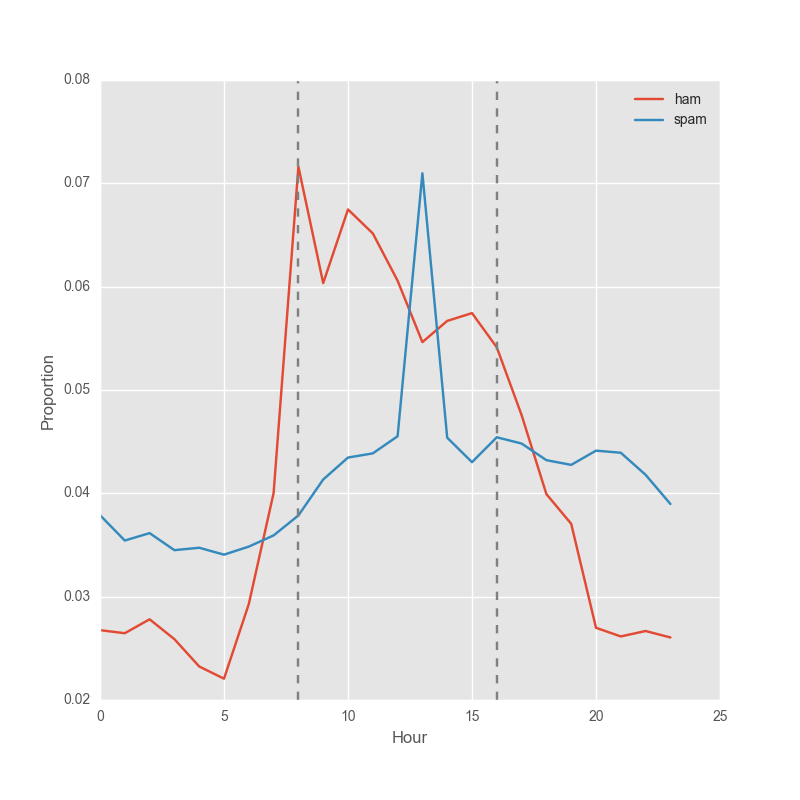
\includegraphics[width=.4\linewidth]{Ham_and_Spam_per_hour.png}
  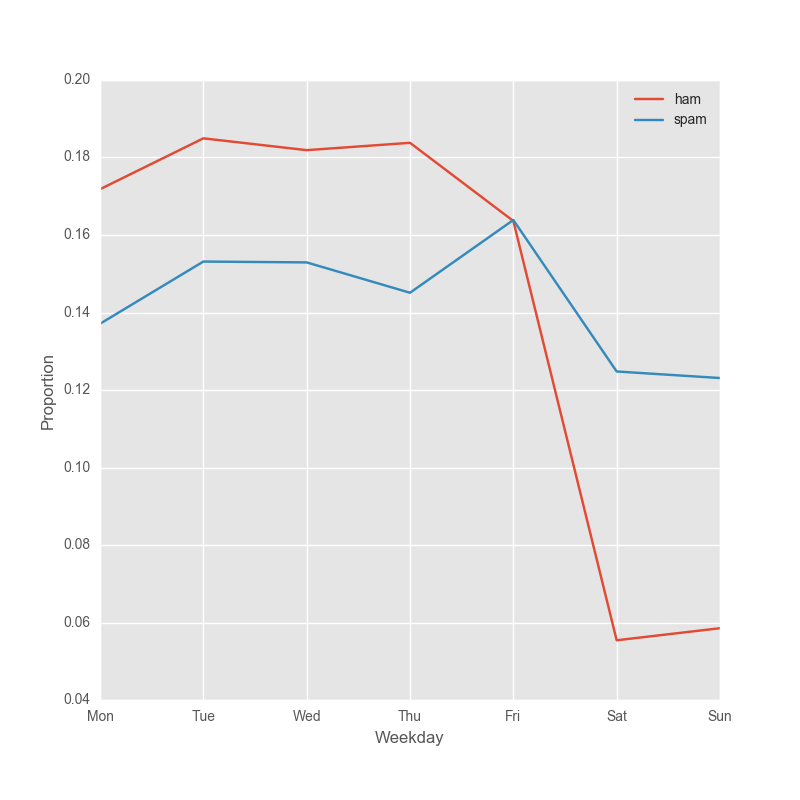
\includegraphics[width=.4\linewidth]{Ham_and_Spam_weekday.png}\\
\end{subfigure}%
\caption{Amount of Email Hourly and On Different Weekday}
\label{email_hour_weekday}
\end{figure}

\subsection{Top 10 Words Per Year}

% !TEX root = main.tex

One of the main purposes for this project is to explore whether the keywords for spam and ham email changed by year. In this section, we counted the appear frequency of each word as a vector by year respectively. Sort the frequency and find out the top 10 frequent words per year. We would like to explore that whether the frequent words changed by year. Moreover, in the next section, we will use word cloud to visualize the results we found out.\\

According to the Figure.\ref{topwordspam}, although keywords did not change year by year, we still have found out that there might have a difference in 2002. Before 2001, some keywords appreared repeatedly, such as "microsoft", "adobe", "windows", and "free". It seems before 2001, in our data set, the spam emails mostly are related to computer and Microsoft topics. From 2002, "stock", "business", "money", and  "com" become top frequent keywords. We categorize those as economy and Internet topics. \\

For the ham email (Figure. \ref{topwordham}), there is not specific topic for each year. We cannot conclude any specific topic or gap for year. However, overall keywords mainly focus on acadmic, such as "edu", "university", "data". We inferred that ham email data may mostly come from academic organizations.\\

\begin{figure}[H]
    \centering
    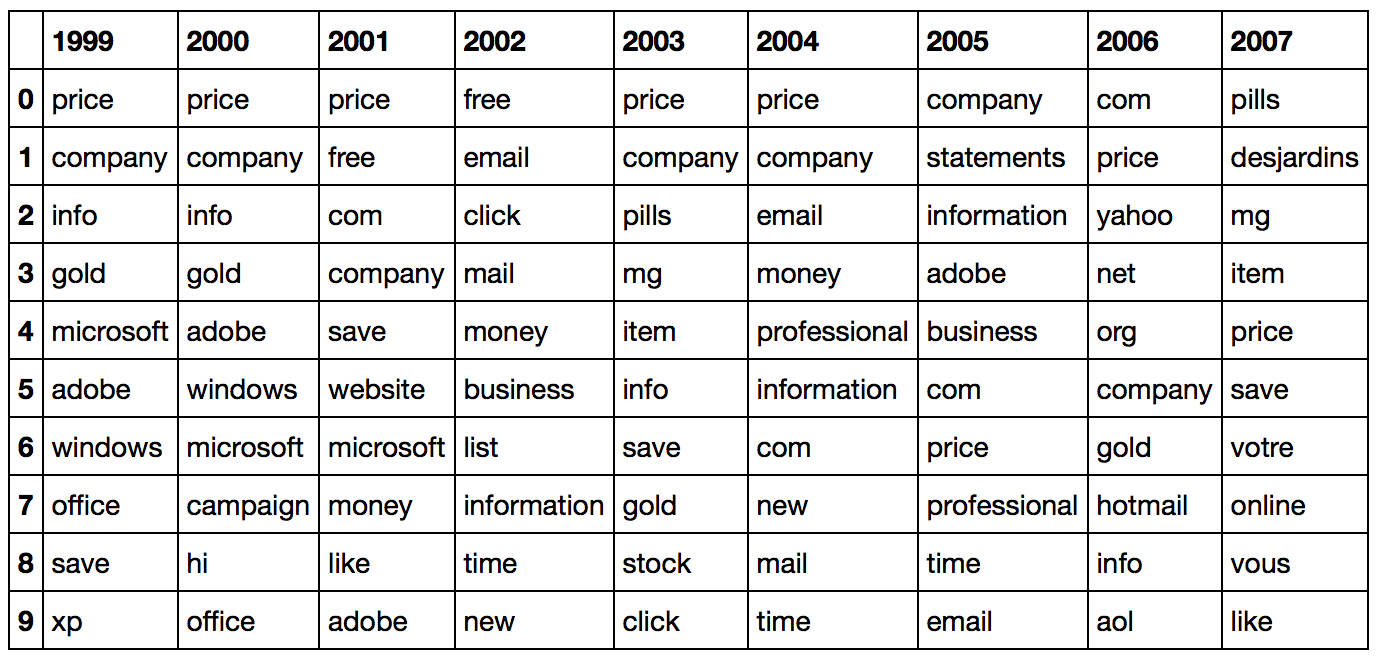
\includegraphics[width=13cm]{./plots/top_word_spam.png}
    \caption{Top 10 Frequent Words Of Spam Email}
    \label{topwordspam}
\end{figure}


\begin{figure}[H]
    \centering
    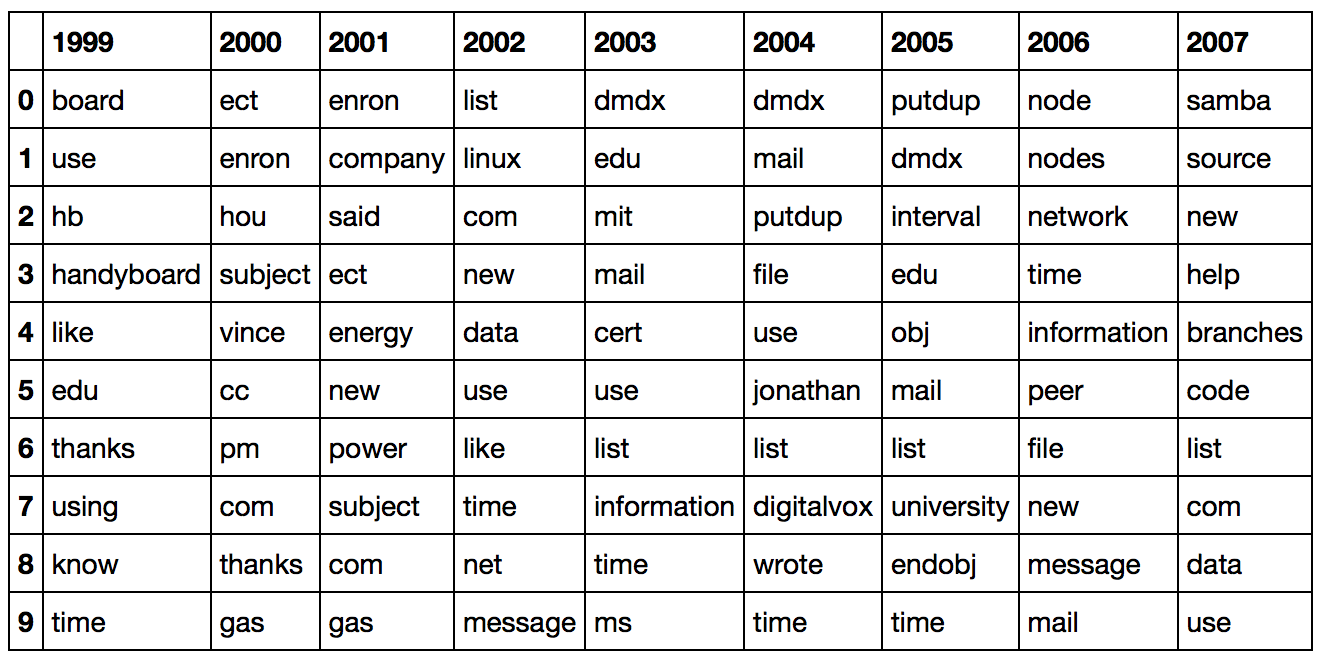
\includegraphics[width=13cm]{./plots/top_word_ham.png}
    \caption{Top 10 Frequent Words Of Ham Email}
    \label{topwordham}
\end{figure}




\subsection{Word Cloud}
% !TEX root = main.tex
\vskip -2ex

\begin{figure}[H]
\begin{subfigure}{\textwidth}
  \centering
  \includegraphics[width=.4\linewidth]{{"./plots/wordCloudImages/Ham 1999"}.png}
  \includegraphics[width=.4\linewidth]{{"./plots/wordCloudImages/Spam 1999"}.png} \\
  
   \vskip -7ex
   
   \includegraphics[width=.4\linewidth]{{"./plots/wordCloudImages/Ham 2000"}.png}
  \includegraphics[width=.4\linewidth]{{"./plots/wordCloudImages/Spam 2000"}.png} \\
  
  \vskip -7ex
    
  \includegraphics[width=.4\linewidth]{{"./plots/wordCloudImages/Ham 2001"}.png}
  \includegraphics[width=.4\linewidth]{{"./plots/wordCloudImages/Spam 2001"}.png} \\ 
  
  \vskip -7ex
  
   \includegraphics[width=.4\linewidth]{{"./plots/wordCloudImages/Ham 2002"}.png}
  \includegraphics[width=.4\linewidth]{{"./plots/wordCloudImages/Spam 2002"}.png} \\ 
  
  \vskip -7ex
  
    \includegraphics[width=.4\linewidth]{{"./plots/wordCloudImages/Ham 2003"}.png}
  \includegraphics[width=.4\linewidth]{{"./plots/wordCloudImages/Spam 2003"}.png} \\ 
  
  \vskip -7ex
  
  \includegraphics[width=.4\linewidth]{{"./plots/wordCloudImages/Ham 2004"}.png}
  \includegraphics[width=.4\linewidth]{{"./plots/wordCloudImages/Spam 2004"}.png} \\   
  
\end{subfigure}%
\caption{Word Cloud For Spam And Ham Email From 1999 to 2004}
\end{figure}

\begin{figure}[H]
\begin{subfigure}{\textwidth}
\centering
  
  \includegraphics[width=.4\linewidth]{{"./plots/wordCloudImages/Ham 2005"}.png}
  \includegraphics[width=.4\linewidth]{{"./plots/wordCloudImages/Spam 2005"}.png} \\ 
  
  \vskip -7ex
  
  \includegraphics[width=.4\linewidth]{{"./plots/wordCloudImages/Ham 2006"}.png}
  \includegraphics[width=.4\linewidth]{{"./plots/wordCloudImages/Spam 2006"}.png} \\ 
  
  \vskip -7ex
  
  \includegraphics[width=.4\linewidth]{{"./plots/wordCloudImages/Ham 2007"}.png}
  \includegraphics[width=.4\linewidth]{{"./plots/wordCloudImages/Spam 2007"}.png} 
  
\end{subfigure}%
\caption{Word Cloud For Spam And Ham Email From 2005 to 2007}
\end{figure}

From the wordclouds, we see that Microsoft and windows XP seem to be a consistent theme in spam. However, we do see a shift less on windows and more towards sales and products during the later half. For ham, based on the words that show up, we may think that the email data originate from an education or technical source due to terms like edu and systems. \\


\section{Previous Studies}

\section{Method}

\subsection{Feature Engineering}

\subsection{Fit Models}

\subsection{Conclusion and exploration}


\end{document}